%\twocolumn[
%\begin{@twocolumnfalse}
\bbook{The Book of Whimsy}{and also Pranks and Monkeys and Such.}
\begin{center}
\booktitlefont\textsc{argvment.}
\end{center}
\begin{center}
\parbox{4.67in}{%
\begin{bookcomment}
Whimsy was defined by someone somewhere as ``a thing that is fanciful or odd,'' and probably comes from the word whim-wham, which doesn't mean much of anything.

This Book celebrates the Pranksters and the Tricksters, the Circus Folk, the Dancers, and Hey\'ok\v{h}a.\\

\bigskip
\begin{center}
It is Your Book!\\
Not just to look\\
Yours to decorate\\
And recreate,\\
Yours to re-make\\
But (please) not Yours to Take.
\end{center}
\end{bookcomment}
}
\end{center}
%\end{@twocolumnfalse}
%]
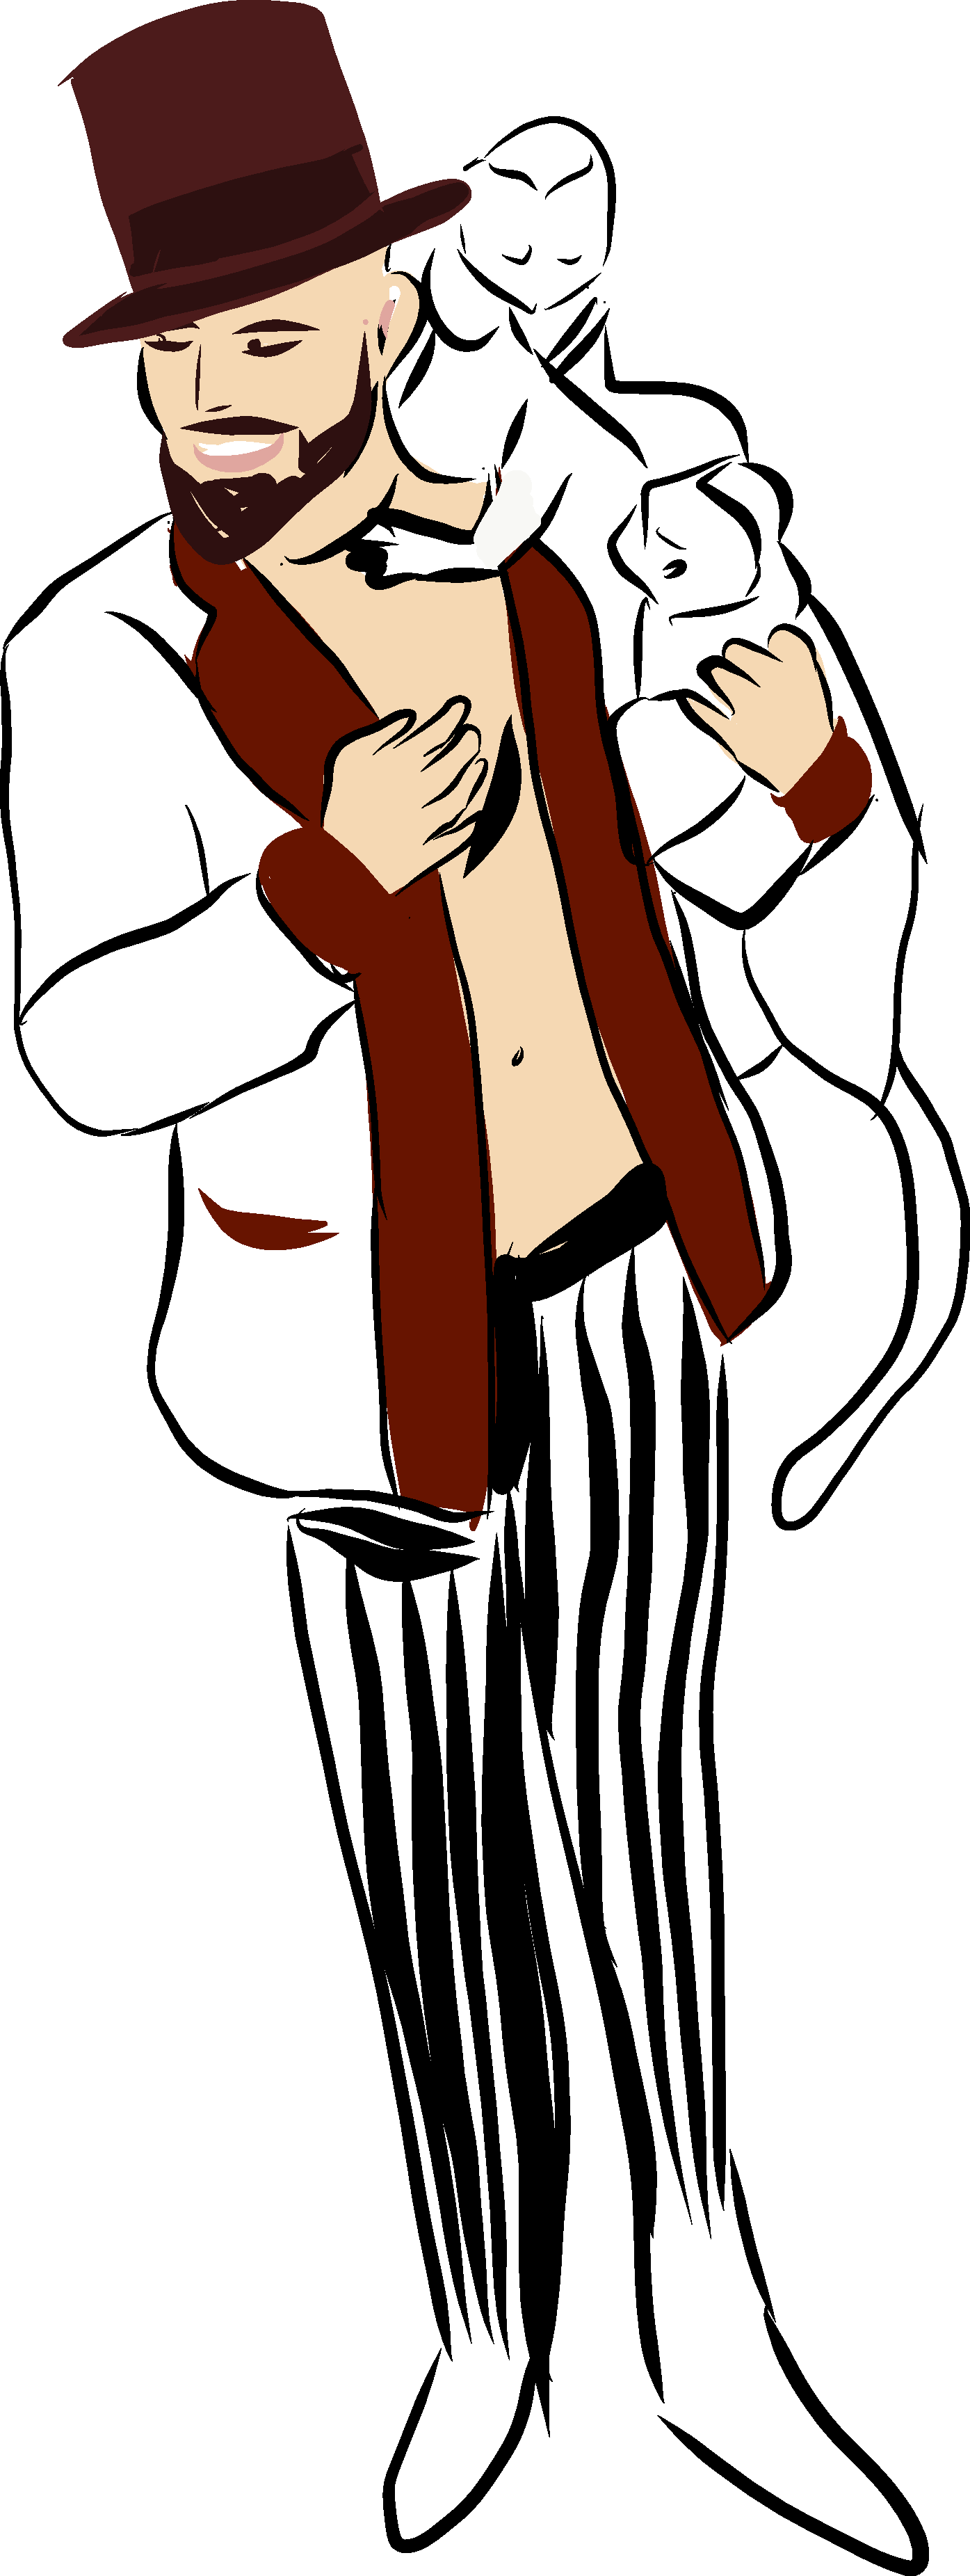
\includegraphics[width=2in]{images/monkey_circus.pdf}
%\begin{@twocolumnfalse}
\hbox{\footnotesize{``Why wouldn't you finish my shoes?''}}
%\end{@twocolumnfalse}
\clearpage
\clearpage
%\onecolumn[
\bversenonum \firstletter{I}{f you were a deity}, what prank would you play on your followers?
%]
\clearpage
\clearpage
\bversenonum \firstletter{W}{rite} a series of haikus describing the messiah of clowns (not the creepy kind).
\clearpage
\clearpage
\bversenonum \firstletter{D}{ancing} is a moral act \textit{because}
\clearpage
\clearpage
\bversenonum \firstletter{I}{f you were a deity}, what would you juggle --- planets? angels? souls? jugglers? --- and why?
\clearpage
\clearpage
\bversenonum \firstletter{T}{ell the story} of the God of Hot Air Balloons (and Dirigibles).
\clearpage
\clearpage
\bversenonum \firstletter{M}{ake} up, and draw a picture of, a hybrid between two mythical animals, or create an entirely new animal.
\\
\\
\\
\\
\\
\bverse Let someone else tell this new animal's story.
\bverse Where does it snorgleblast?
\bverse How does it sex?
\bverse What hijinks does it get up to?
\bverse How does it feel about space travel?
\bverse Can it science?
\clearpage
\clearpage
\bversenonum \firstletter{B}{lessed} are the thespians, for they\\
\\
\\
\\
\\
\bverse Blessed are the aerialists, for\\
\\
\bverse Blessed are the stiltwalkers, \\
\\
\bverse Blessed are the fire-spinners, \\
\\
\bverse Blessed are the lindy hoppers, \\
\\
\bverse Blessed are the pop-lockers, \\
\\
\bverse Blessed are the break dancers, \\
\\
\bverse Blessed are the burlesque performers, \\
\\
\bverse Blessed are the Vaudivillians (and Vaudivillains), \\
\\
\bverse Blessed are the [non-creepy] clowns, \\
\\
\bverse Blessed are the mimes, \\
\\
\bverse Blessed are the non-sequiturs, \\
\\
\bverse Blessed are the illusionists, \\
\\
\bverse Blessed are the political cartoonists, \\
\clearpage
\clearpage
\bversenonum \firstletter{W}{rite} a parable about unicorns.
\clearpage
\clearpage
\bversenonum \firstletter{W}{hat} are the `Ten Commandments' of Whimsy?
\clearpage
\clearpage
%\end{@twocolumnfalse}